\section{Implementation}

\subsection{Systems Architecture \& Description}

\begin{figure}[H]
	\centering
	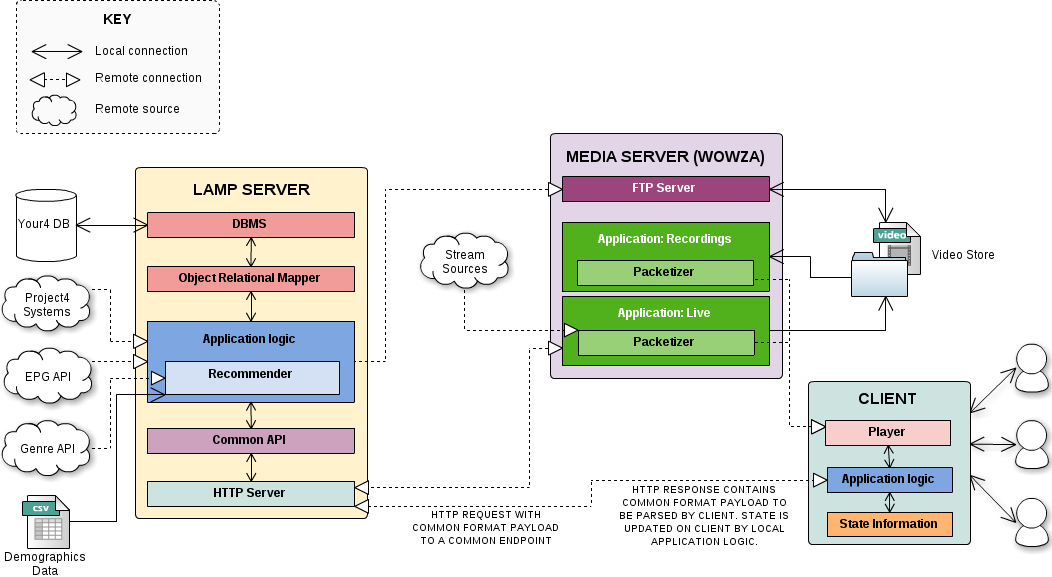
\includegraphics[scale=0.4]{images/your4-architecture.png}
	\caption{Overview of Your4 architecture}
	\label{your4-architecture}
\end{figure}

Figure~\ref{your4-architecture} shows the overall architecture of the Your4 system. The system is split into three distinct parts:

\begin{description}
	\item[Client] The client (expected to be Mobile Safari for iPad running on top of iOS 5+) is responsible for for interfacing with the LAMP server to retrieve the users' personalised playlist. With this playlist, the player in the client can then request the appropriate media from the media server.
	\item[LAMP server] The LAMP server represents the bulk of the system and is responsible for providing a REST API for the key features of Your4: recommendations, user authentication, electronic programme guide (EPG) data and advert uploading \& manipulation.
	\item[Media server] The media server is responsible for encoding and serving live streams as well as recording programmes and serving recorded programmes.
\end{description}

\subsubsection{Client}

The client receives all HTML content from the LAMP server upon the first visit of your4.tv. From this point onwards, all communication between the client and LAMP server contains only models and collections (e.g. a programme and all of its attributes) on the LAMP servers REST interface in JSON format. The client side application is then responsible for parsing this JSON response and manipulating the user interface using local templates (embedded in the HTML upon the initial page load) as appropriate. Due to the asynchronicity this approach brings, a significant UI speed increase can be observed against traditional methods whereby the web browser acts as a ``thin client'', by simply parsing and rendering HTML responses pre-generated server side.

Using the POST, GET, PUT and DELETE methods in HTTP requests to the REST endpoint maps to the equivalent CRUD (create, read, update and delete) operations on the object concerned. This methodology creates a simple self-documenting API. In a similar exploitation of HTTP philosophies, HTTP status codes are used to identify the status of a request. For example, 200 indicates success and 400 indicates the request was invalid (failed server side validation). The client can then perform the appropriate callback function to manipulate the interface.

\paragraph{Authentication}

The concept of a ``user'' is key to the system since crucial demographics data and matrices defining recommender state are stored against each user. The client authenticates a user by either local login or using the Facebook login API\footnote{\footurl{https://developers.facebook.com/docs/concepts/login}}. Upon page load, the client attempts to retrieve ``/api/users/me'' from the server to discover if an active session is available. If so, the player layers will be rendered on screen, otherwise, the user will be routed to the login interface.

The user can then choose to use the local login which will generate a GET request with the email and password as query parameters. If a 200 response is received, the login is considered to be successful. A user can also choose to login via Facebook. After the user accepts the Facebook permissions, a local cookie is set and a GET request is generated to ``/api/users/fb-[facebook\_id]'' where ``[facebook\_id]'' is retrieved from the Facebook API.

\paragraph{Playback}

Upon initialisation of the player, a number of layers are rendered on top of one another:

\begin{description}
	\item[Video layer] The video component to show video. If on an Apple device, this is a HTML5 video tag. Otherwise, a flash video player is instantiated.
	\item[Skip layer] Contains user controls to skip and rate currently playing media.
	\item[Black layer] Used to hide buffering video in order to provide more seamless stream.
	\item[Overlay layer] An iFrame which displays the HTML that the advertiser has specified to be overlayed on their advert.
\end{description}

Once rendering is complete, the client requests a number of resources from the REST API in order to compile and play a playlist:

\begin{enumerate}
	\item A list of channels including the relevant stream URL to the media server.
	\item The current LAMP server timestamp. This is used in recommendation requests.
	\item A request is made for the best recommended live broadcast. This recommendation is based on the currently playing program on each channel. Live broadcasts are given priority over recorded programmes as this is close to the ``personal TV channel'' ideal. The current timestamp and user ID is sent with this request in order for the server to determine what suitable programmes are upcoming. If a 200 response is received, the body will include the channel ID. If a 404 is received, no appropriate live broadcast recommendation is available. The client will then request a recorded programme recommendation. In both cases, the response also includes the programme ID from the EPG and the location of ad breaks.
	\item With the programme ID, a request is made to retrieve the programme data such as name, description and length.
	\item Between each recorded programme a 2 minute ad break is artificially included. Up to 5 minutes is allowed between live broadcasts (depending on previous programme end and the start of the live broadcast). The system is also aware of ad breaks in programmes within the playlist. For each ad break, a request is made containing: the user ID; programme ID; the amount of time in the ad break; if the ad break is between a live or recorded programme and finally, a list of advert ID's which have already been listed in the playlist. Using this data, the LAMP server can select adverts that match the users demographics and the currently playing programme. This step is repeated multiple times, reducing the amount of time left unallocated in the request each time, until all ad breaks are full.
	\item Steps 3 to 5 are repeated until the minimum duration and size of playlist are both satisfied. Upon each repeat, the timestamp sent with the request is set to the end time of the previously recommended programme or advert. This informs the recommender as to the point in time it should check live broadcasts for suitable programmes.
	\item The playlist is rendered on screen.
	\item The video player is instructed to play the first stream URL in the playlist. Each time an item in the playlist ends, a signal is triggered which causes the player to play the next stream. As well as this, another recommendation is requested and added to the playlist.
\end{enumerate}

The client checks the user agent string of the browser to determine what format of media to request from the media server. Apple devices require HTTP Live Streaming (HLS) streams while the flash player alternative requests an RTMP alternative.

\subsubsection{LAMP Server}

\paragraph{Advert selection}
\paragraph{REST Interface}
\paragraph{Recommender}
\paragraph{Data visualisation}
\subsubsection{Media Server}

\subsection{Database structure}


\subsection{Languages and Techniques}
As this project involved interacting with many different systems, a diverse range of programming languages were used.


Communication between server and client is done through a REST interface.

Datebase is MySQL.


\subsubsection{Libraries and Frameworks}



\subsection{Code Statistics}
Lines of code in JS, PHP, Java, Python, HTML, CSS etc

\subsection{System walkthrough}
\begin{figure}[th]
	\centering
	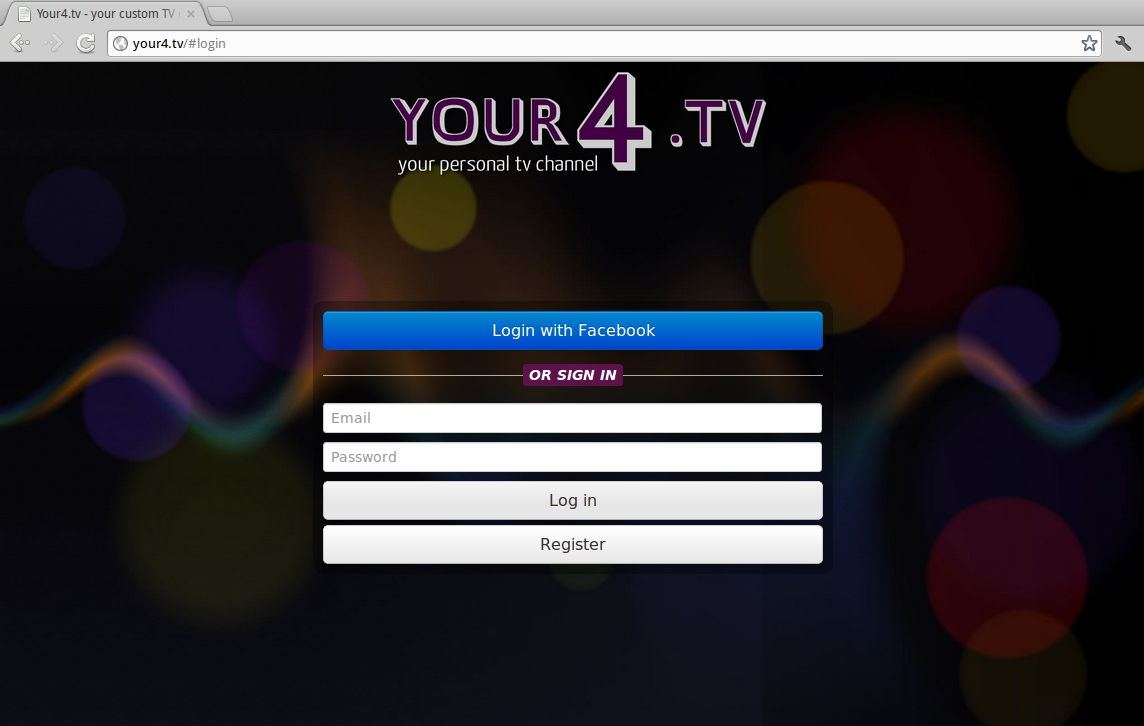
\includegraphics[width=\textwidth]{images/screenshots/your4-login.png}
	\caption{Log in}
	\label{fig:your4-login}
\end{figure}
\begin{figure}[th]
	\centering
	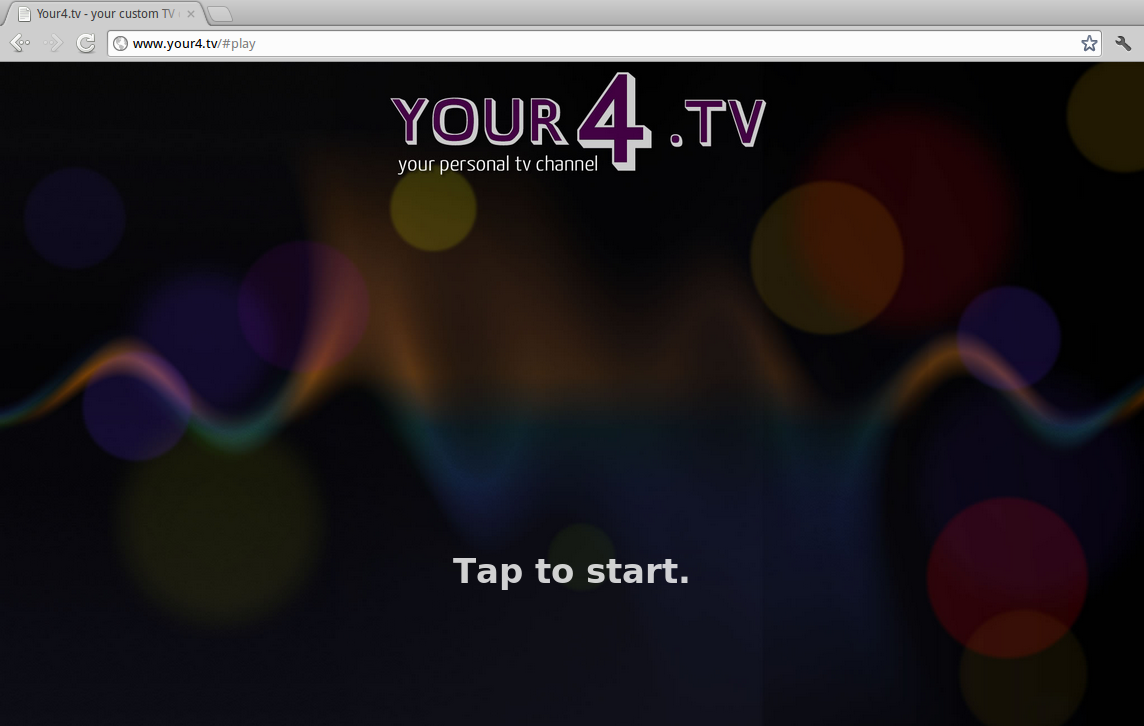
\includegraphics[width=\textwidth]{images/screenshots/your4-tap-to-start.png}
	\caption{Log in}
	\label{fig:your4-tap-to-start}
\end{figure}
\begin{figure}[th]
	\centering
	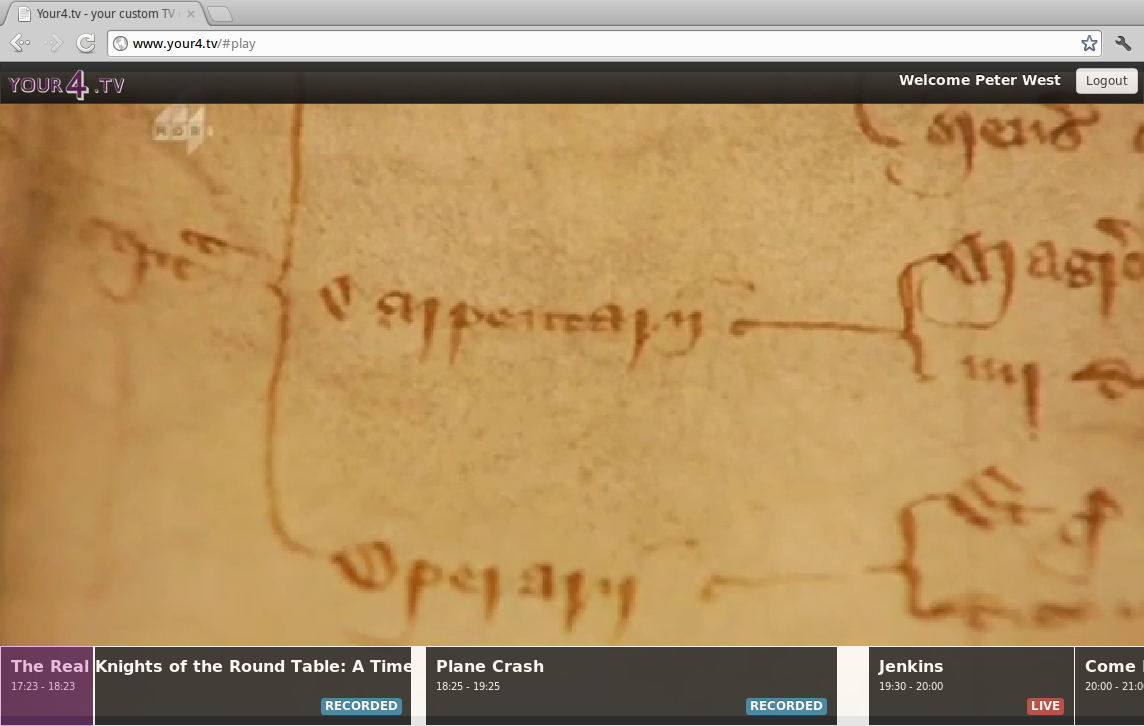
\includegraphics[width=\textwidth]{images/screenshots/your4-play.png}
	\caption{Log in}
	\label{fig:your4-play}
\end{figure}

\begin{figure}[th]
	\centering
	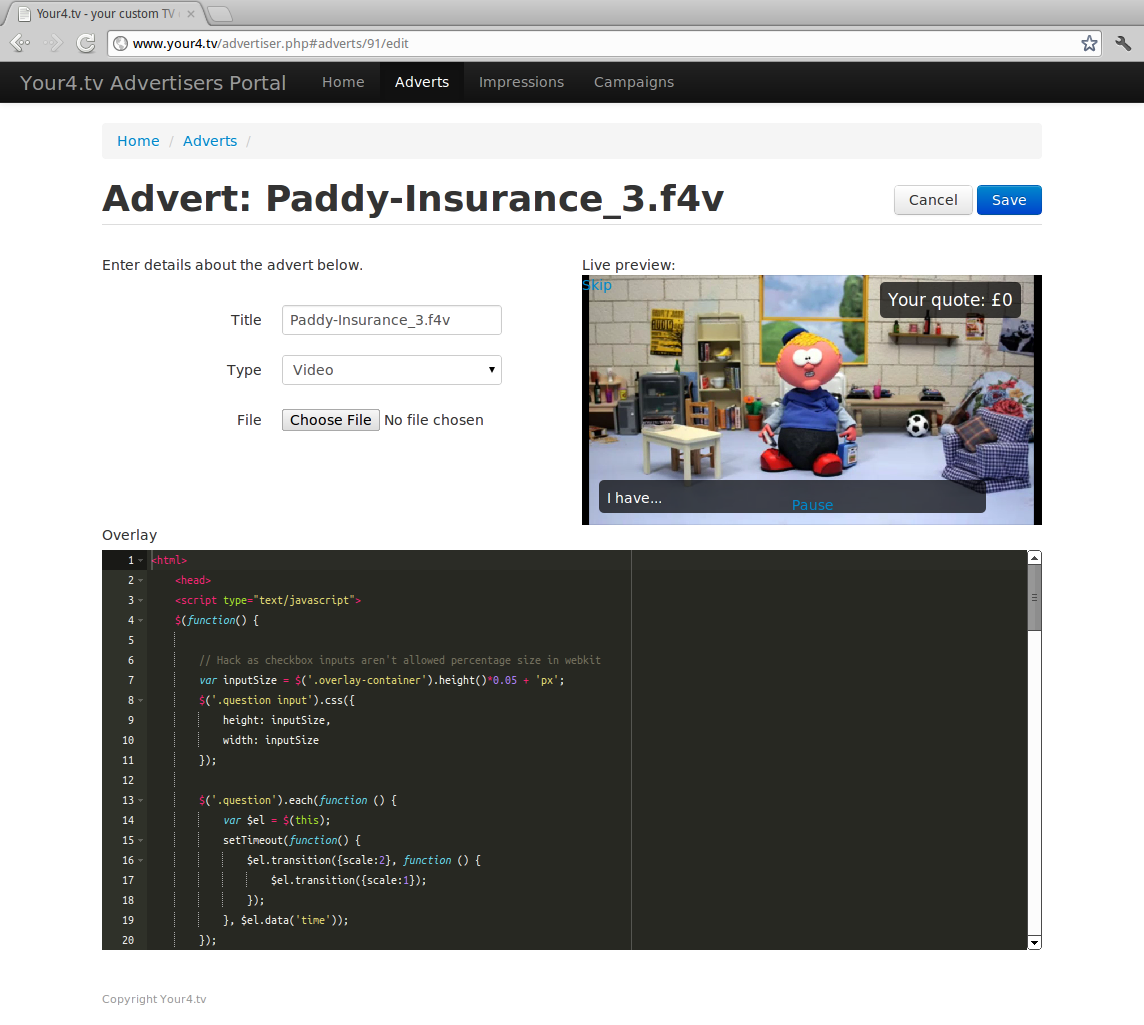
\includegraphics[width=\textwidth]{images/screenshots/advertiser-advert-edit.png}
	\caption{Log in}
	\label{fig:advertiser-advert-edit}
\end{figure}
\begin{figure}[th]
	\centering
	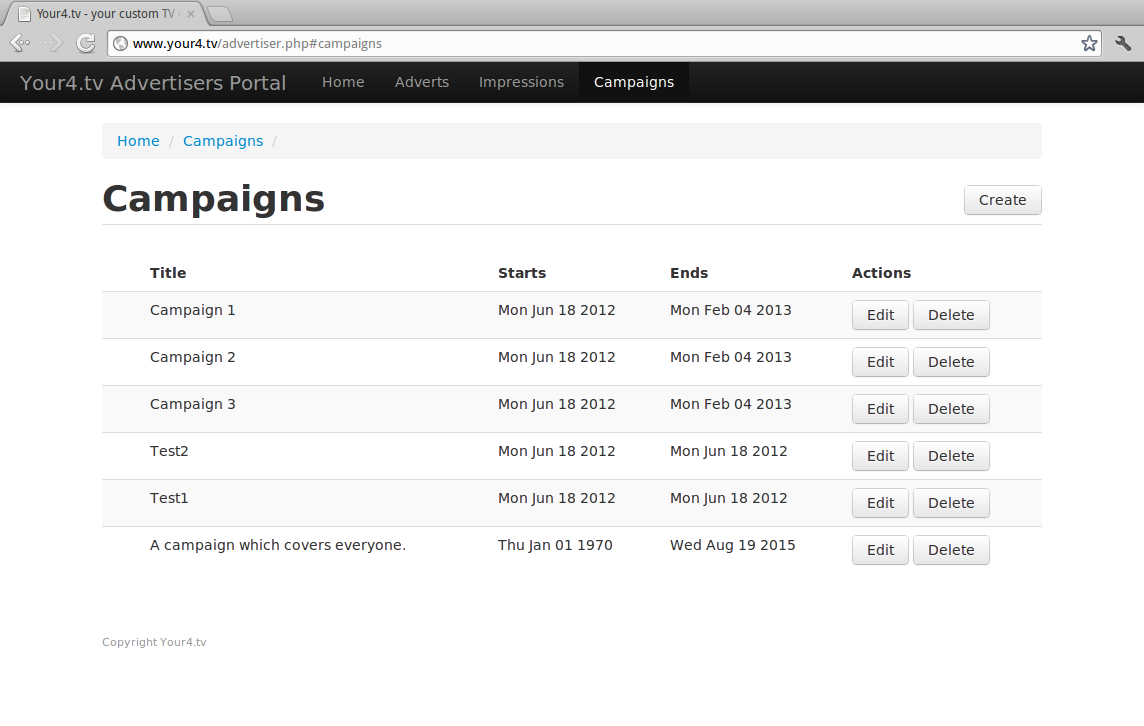
\includegraphics[width=\textwidth]{images/screenshots/advertiser-campaigns.png}
	\caption{Log in}
	\label{fig:advertiser-campaigns}
\end{figure}
\begin{figure}[th]
	\centering
	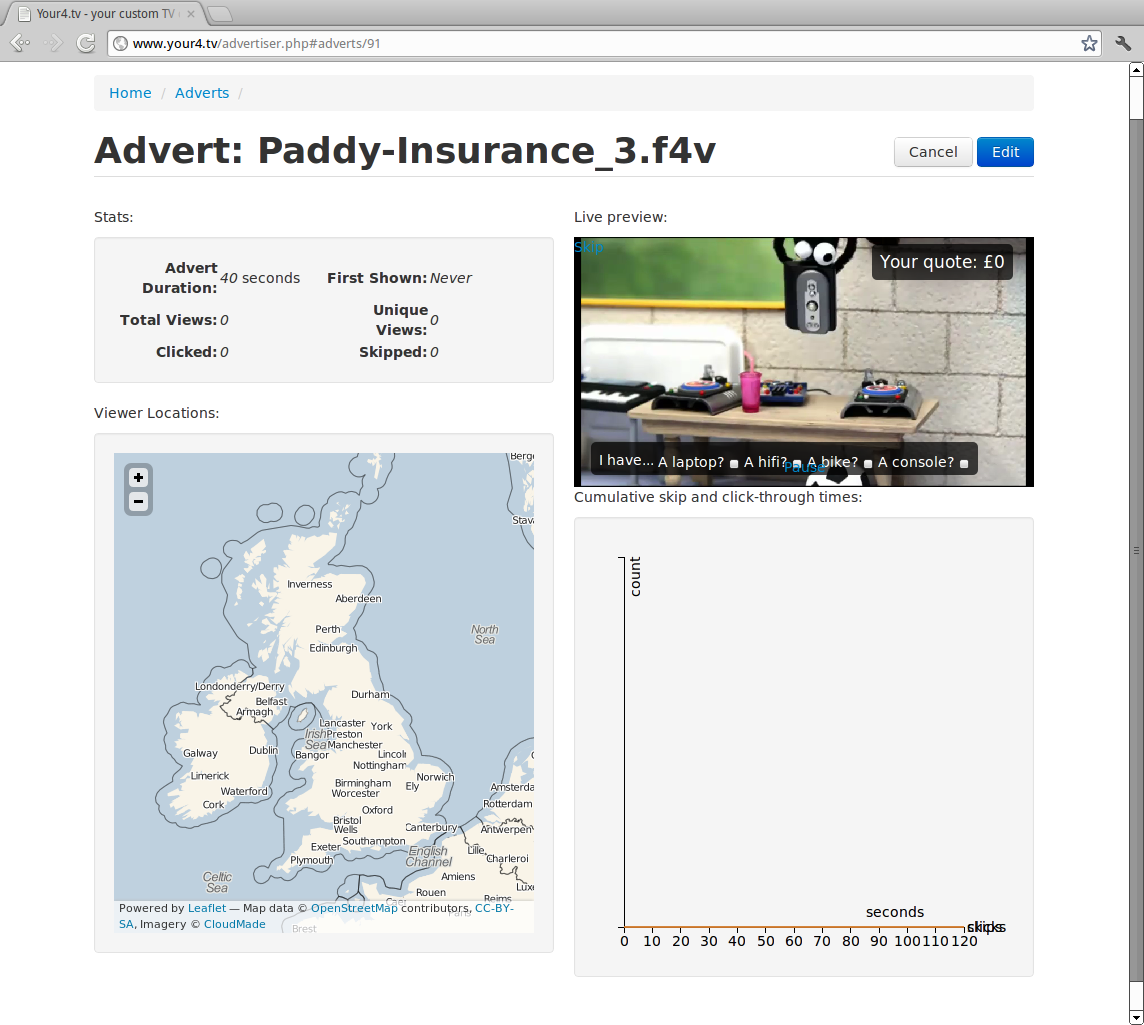
\includegraphics[width=\textwidth]{images/screenshots/advertiser-advert.png}
	\caption{Log in}
	\label{fig:advertiser-advert}
\end{figure}
\begin{figure}[th]
	\centering
	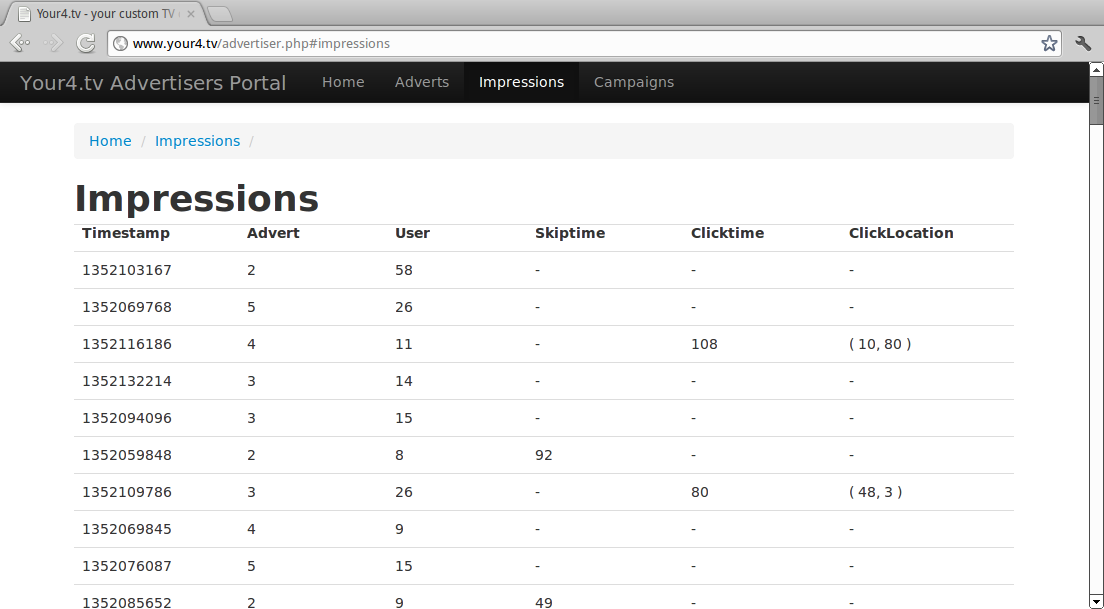
\includegraphics[width=\textwidth]{images/screenshots/advertiser-impressions.png}
	\caption{Log in}
	\label{fig:advertiser-impressions}
\end{figure}
\begin{figure}[th]
	\centering
	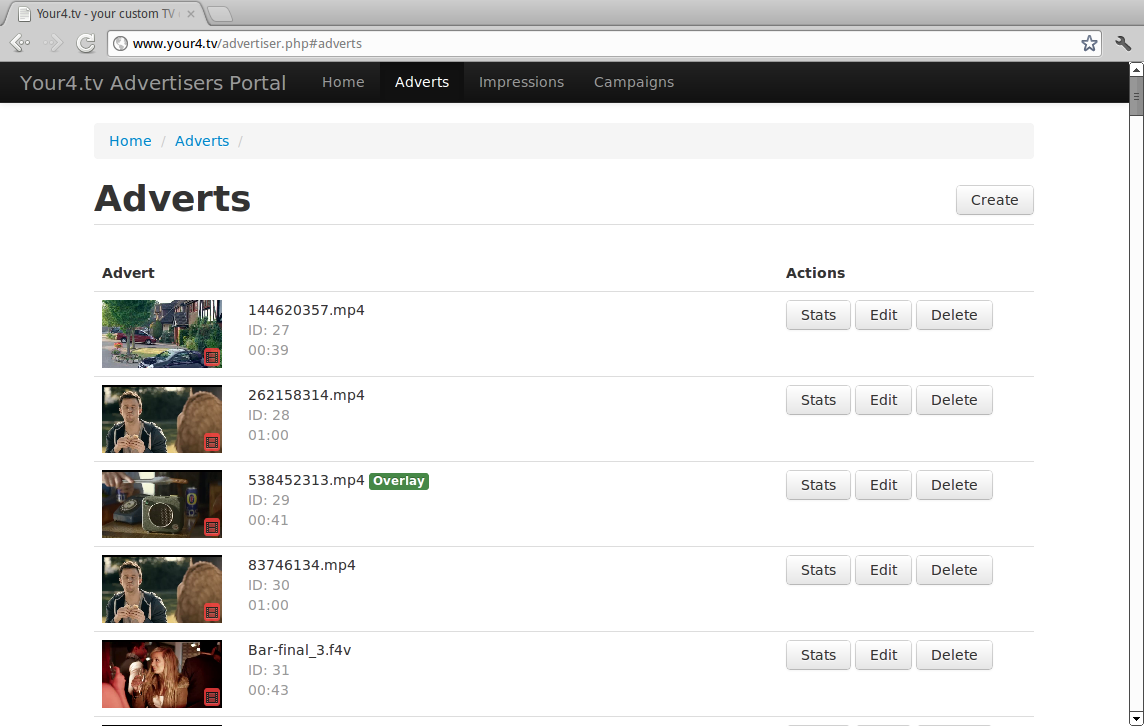
\includegraphics[width=\textwidth]{images/screenshots/advertiser-adverts.png}
	\caption{Log in}
	\label{fig:advertiser-adverts}
\end{figure}
\begin{figure}[th]
	\centering
	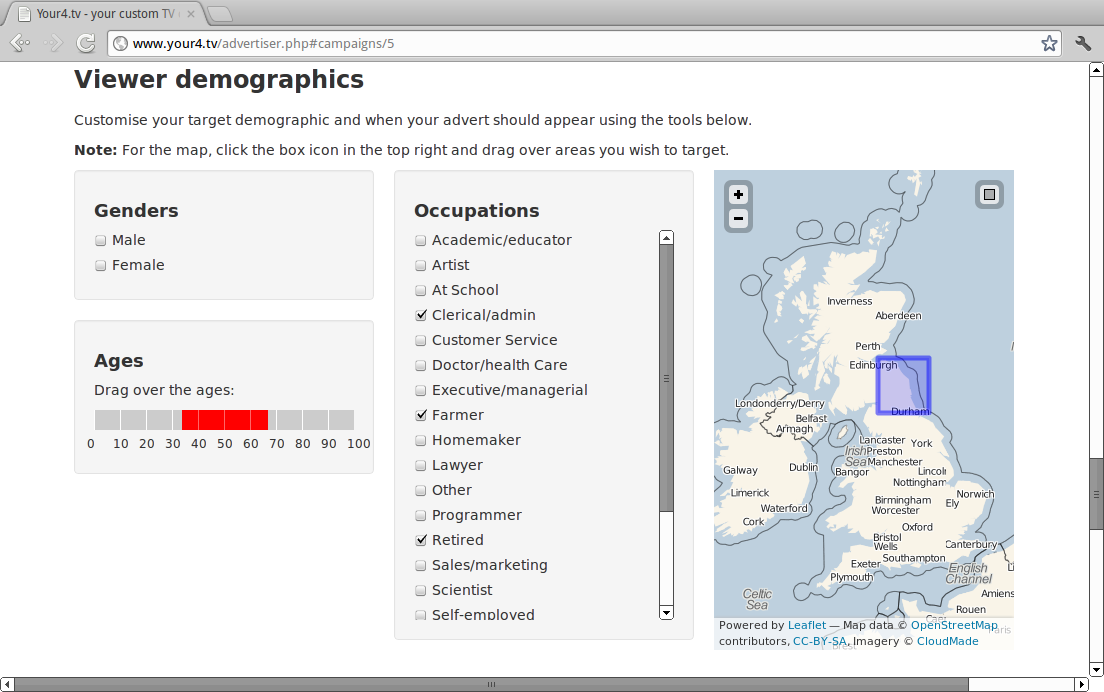
\includegraphics[width=\textwidth]{images/screenshots/advertiser-campaign-demographics.png}
	\caption{Log in}
	\label{fig:advertiser-campaign-demographics}
\end{figure}
\begin{figure}[th]
	\centering
	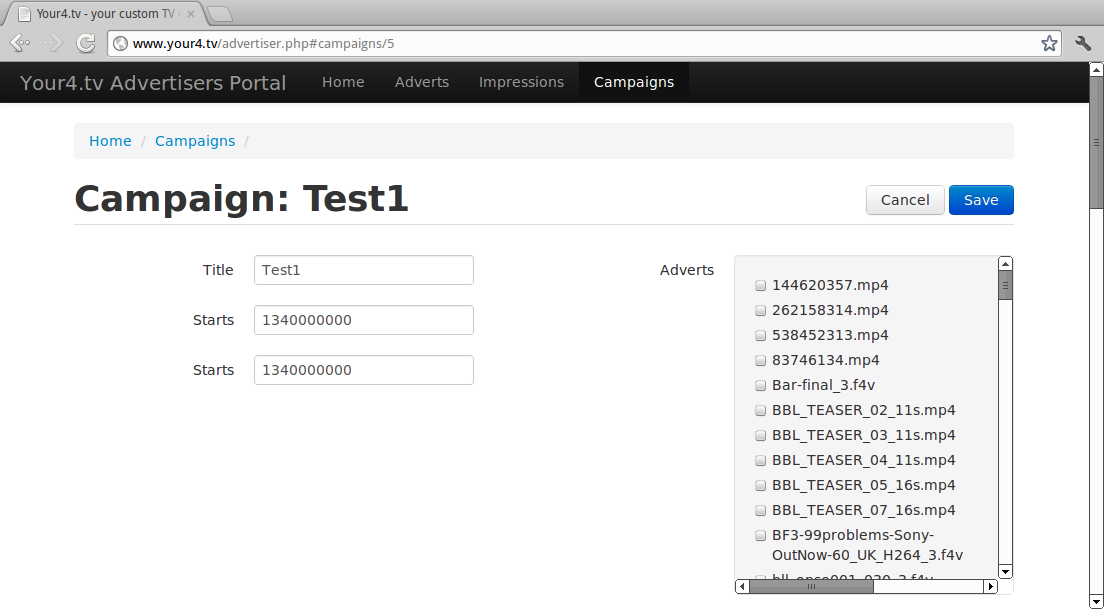
\includegraphics[width=\textwidth]{images/screenshots/advertiser-campaign.png}
	\caption{Log in}
	\label{fig:advertiser-campaign}
\end{figure}
\begin{figure}[th]
	\centering
	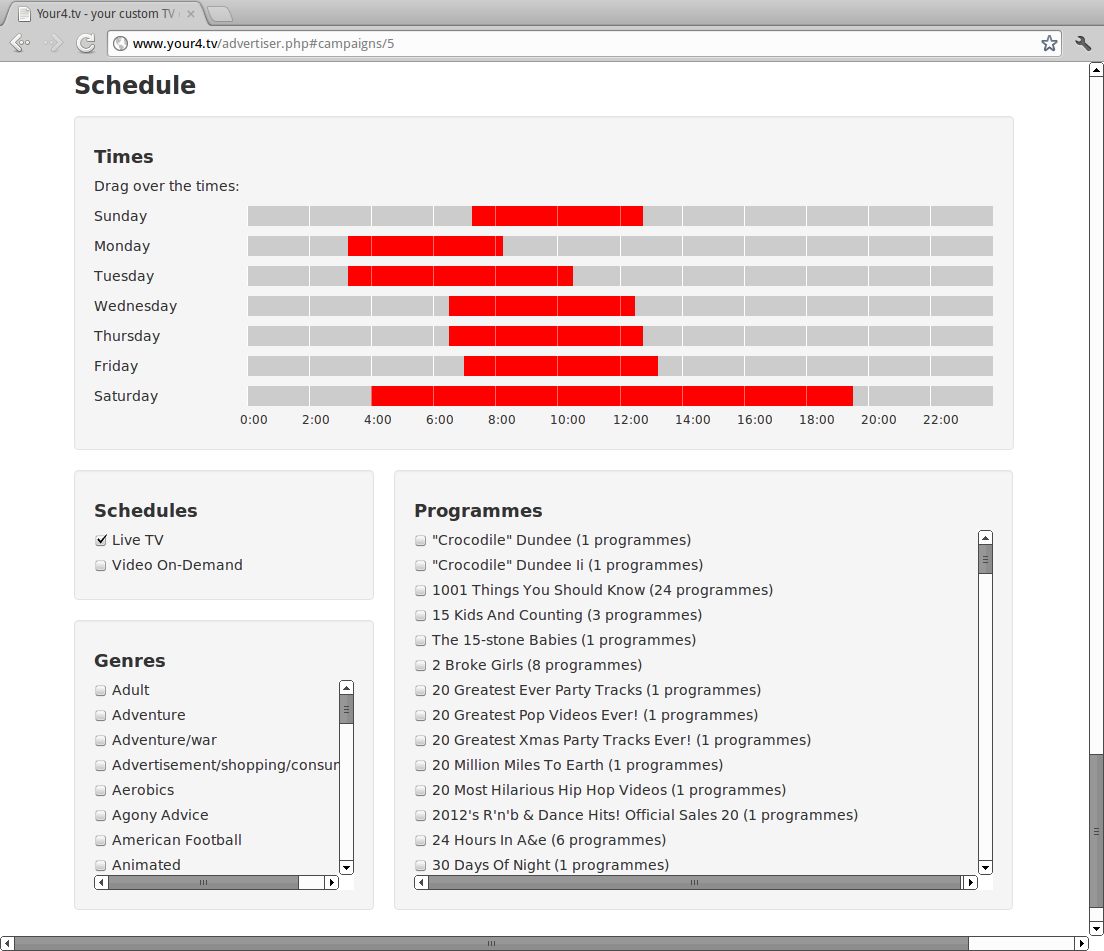
\includegraphics[width=\textwidth]{images/screenshots/advertiser-campaign-schedule.png}
	\caption{Log in}
	\label{fig:advertiser-campaign-schedule}
\end{figure}